\documentclass[a4paper]{article}
\usepackage[utf8]{inputenc}
\usepackage[T1]{fontenc}
\usepackage[french]{babel}
\usepackage{geometry}
\geometry{hmargin=3cm,vmargin=3cm}
\usepackage{graphicx}
\usepackage{fancyhdr}
\usepackage{color}

\usepackage{listings}
\lstset{ %
  backgroundcolor=\color{white},   % choose the background color; you must add \usepackage{color} or \usepackage{xcolor}
  basicstyle=\small,               % the size of the fonts that are used for the code
  breakatwhitespace=false,         % sets if automatic breaks should only happen at whitespace
  breaklines=true,                 % sets automatic line breaking
  captionpos=b,                    % sets the caption-position to bottom
  commentstyle=\color{green},      % comment style
  deletekeywords={...},            % if you want to delete keywords from the given language
  escapeinside={\%*}{*)},          % if you want to add LaTeX within your code
  extendedchars=true,              % lets you use non-ASCII characters; for 8-bits encodings only, does not work with UTF-8
  frame=single,                    % adds a frame around the code
  keepspaces=true,                 % keeps spaces in text, useful for keeping indentation of code (possibly needs columns=flexible)
  keywordstyle=\color{blue},       % keyword style
  language=xml,                    % the language of the code
  morekeywords={Level,Cache,Architecture,...},            % if you want to add more keywords to the set
  numbers=left,                    % where to put the line-numbers; possible values are (none, left, right)
  numbersep=5pt,                   % how far the line-numbers are from the code
  numberstyle=\tiny\color{blue},  % the style that is used for the line-numbers
  rulecolor=\color{black},         % if not set, the frame-color may be changed on line-breaks within not-black text (e.g. comments (green here))
  showspaces=false,                % show spaces everywhere adding particular underscores; it overrides 'showstringspaces'
  showstringspaces=false,          % underline spaces within strings only
  showtabs=false,                  % show tabs within strings adding particular underscores
  stepnumber=2,                    % the step between two line-numbers. If it's 1, each line will be numbered
  stringstyle=\color{red},         % string literal style
  tabsize=2,                       % sets default tabsize to 2 spaces
  title=\lstname                   % show the filename of files included with \lstinputlisting; also try caption instead of title
}
\usepackage{hyperref}
\hypersetup{colorlinks=true}

\pagestyle{fancy}

\lhead{Rapport}
\rhead{Bibliothèque de Threads}
\lfoot{ENSEIRB-MATMECA}
\rfoot{Système d'Exploitation 2013-2014}

\begin{document}

\thispagestyle{empty}

\vspace{\stretch{1}}
\hrule
\begin{flushleft}
\Huge{Bibliothèque de Threads}\\
\end{flushleft}
\begin{flushright}
\huge\textbf{Rapport}\\
\end{flushright}
\hrule

\vspace{\stretch{1}}
\noindent\textbf{Auteurs :}
\emph{BOURDEAU Thibaud, DANDO Louis-Marie, HONORAT Alexandre, RINCEL Guillaume, SAGARDIA Elorri}\\
\\
\noindent\textbf{Encadrant :}
\emph{M. FAVERGE Mathieu}\\
\\
\noindent\textbf{Enseignant :}
\emph{M. GOGLIN Brice} 

\vspace{\stretch{1}}
\normalsize
\begin{center}
  Deuxième année, filière informatique\\
  Date : \today\\
  \textsc{Enseirb-Matmeca}
\end{center}


\newpage
%\tableofcontents

%\vspace{0.2\textheight}

\section*{Introduction}

\paragraph{}
Le projet de système d'exploitation consiste à développer une bibliothèque de threads, basée sur l'interface de \texttt{p\_thread}. Il s'agit dans cette version de la création de \emph{threads} utilisateurs uniquement, tous sur le même thread noyau ; ainsi tous les threads que créera l'utilisateur seront exécutés de manière séquentielle.

\paragraph{}
L'objectif était de pouvoir implémenter toutes les fonctions de prototypes identiques à ceux de \texttt{p\_thread}, de sorte que tous les tests fournis fonctionnent. Ce rapport présente l'aboutissement de ce projet, divisé en plusieurs parties : la première concerne l'implémentation initiale afin de passer les tests fournis, puis les suivantes décrivent les fonctionnalités avancées que nous avons développées pour améliorer cette première version.

\newpage

\section{Fonctionnement de la bibliothèque}

 La bibliothèque, s'inspirant de \texttt{p\_thread}, implémente les
fonctions suivantes:
\begin{itemize}
  \item \texttt{thread\_self}
  \item \texttt{thread\_create}
  \item \texttt{thread\_yield}
  \item \texttt{thread\_join}
  \item \texttt{thread\_exit}
\end{itemize}

\subsection{Organisation des sources}

\paragraph{} L'implémentation de ces fonctions requiert la définition
de certaines structures regroupées dans le répertoire
\texttt{src/includes}. Les principales structures sont :
\begin{itemize}
\item La structure de thread.
\item La structure de liste.
\end{itemize} La bibliothèque \texttt{ccan\_list} a été choisie pour
représenter les listes. Mais afin de pouvoir adapter le code à un
autre type de liste, des fonctions d'abstraction ont été écrites dans
\texttt{src/others/manip\_list.c}. Celles-ci permettent d'effectuer
les opérations basiques sur les listes : parcours, ajout,
suppression. De même, aucun ordonnanceur -- autre que l'utilisation
basique des listes -- n'est implémenté pour l'instant, mais ses deux
fonctions principales (i.e. l'ajout d'un thread à la liste des threads
en attente ou prêts, ainsi que la récupération du prochain thread à
exécuter) sont regroupées dans un module à part :
\texttt{src/core/ordo.c}.
\paragraph{} Enfin les programmes de tests fournis ont été rassemblés
dans le répertoire \texttt{src/prog\_tests} et le fichier
\texttt{thread.c} a été placé dans le répertoire \texttt{src/core} et
contient le code principal du programme. La bibliothèque dynamique
créée est \texttt{thread.so}, ce qui permet de ne compiler qu'une
seule fois les tests.


\subsection{Choix effectués}

La programmation d'une bibliothèque de threads peut s'effectuer de
nombreuses façons, en effet différentes politiques d'ordonnancement,
de préemption, etc existent. La section suivante précisent ces choix.

\subsubsection{Stockage des threads}

\paragraph{} La manière de stocker les threads en mémoire est
déterminante sur l'ordonnancement. Les threads sont ainsi stockés
selon leur état dans une des trois structures suivantes :
\begin{itemize}
\item la \texttt{waiting\_list}, qui contient les threads ayant
terminé mais n'ayant pas été récupérés par leur parent ;
\item la \texttt{ready\_list}, qui contient la liste des threads prêts
à s'exécuter ;
\item le thread \texttt{running}, qui contient le threads en cours
d'exécution.
\end{itemize} Actuellement, un seul thread noyau est employé pour
exécuter l'ensemble des threads créés par l'utilisateur. L'utilité
d'une liste \texttt{running} ne nous a, par conséquent, pas semblé
nécessaire pour ce thread particulier. Par ailleurs notons que les
deux listes implémentées sont utilisées comme des FIFOs : un thread y
est toujours ajouté à la fin, et c'est le premier qui est récupéré.

\subsubsection{La structure thread}

\paragraph{} Premièrement, un choix s'est imposé sur la définition de
la structure thread. Un thread est de manière évidente, attaché à un
contexte et la structure doit donc le contenir.
\paragraph{} D'autre part, un thread, à chaque instant, est soit en
attente, soit prêt à être executé, soit en execution. Le statut du
thread est stocké au sein de la structure \texttt{thread} elle-même
pour des raisons d'optimisation. En effet, il serait inutilement
coûteux de devoir parcourir chaque liste à la recherche d'un certain
thread pour obtenir son statut, notamment dans le cas d'un
\texttt{join} qui doit vérifier si un thread est dans la
\texttt{waiting\_list}.
\paragraph{} Par ailleurs, au vu du contenu des fonctions de
\texttt{thread.c}, nous avons choisi de marquer le thread du
\texttt{main} d'une manière différente. En effet, son
allocation/desallocation s'effectue distinctement des autres : sa pile
n'est pas allouée par la bibliothèque. Ce marquage se traduit par un
attribut \texttt{is\_main}.
\paragraph{} Enfin, un attribut \texttt{retval} permet le stockage de
la valeur renvoyée au niveau du \texttt{thread\_join}. Pour gérer le
cas d'un thread qui n'appelle pas la fonction \texttt{thread\_exit},
une fonction auxiliaire a été implémentée dans la bibliothèque et
prend comme argument la fonction passée à \texttt{thread\_create}
ainsi que son argument d'appel. Il s'agit d'un \emph{wrapper} qui lui
appelle la fonction \texttt{thread\_exit} dans tous les cas.

\subsubsection{Initialisation et Terminaison}

\paragraph{}
Les fonctions de la bibliothèque nécessitent que
certains objets soient instanciés au préalable. C'est le cas des deux
listes initialisées vides et du thread running qui est initialisé avec le thread du
\texttt{main}. De la même façon, avant de quitter le programme, le
thread running doit être détruit (les listes ready et waiting sont
déjà vides à ce moment là). C'est pourquoi les
fonctions \texttt{thread\_init} et \texttt{thread\_quit} sont
appelées automatiquement car définies avec des attributs
\emph{constructor} et \emph{destructor} respectivement.

\paragraph{}
D'autre part, afin d'éviter la duplication de code, une
fonction d'allocation \texttt{thread\_construct} et de désallocation
\texttt{thread\_destruct} internes au fichier \texttt{thread.c} ont
été ajoutées. La fonction d'allocation est appelée à la fois par
\texttt{thread\_init} et par \texttt{thread\_create} et c'est elle qui
effectuera des traitements différents en fonction du thread (running
et/ou main ou cas général). De la même manière, la fonction de
désallocation peut être appelée par \texttt{thread\_quit} ou
\texttt{thread\_join}. En effet, dès qu'un thread est récupéré par son
parent, il doit être détruit.

\subsubsection{Création de contexte}

\paragraph{}
Le choix entre \texttt{swapcontext} et \texttt{setcontext} dépend du
 besoin de retenir le contexte précédent ou non. C'est ainsi que 
\texttt{thread\_yield} utilise \texttt{swapcontext} alors que 
\texttt{run\_thread}, appelé uniquement lorsque la \texttt{ready\_list}
ne contient qu'un élément, utilise \texttt{setcontext}. 

\subsubsection{Le thread issu de main}

\paragraph{}
Le thread principal est le seul thread que la bibliothèque ne crée
pas : son traitement demande par conséquent quelques adaptations.
En particulier, sa pile n'est pas allouée. Il est donc hors de
question de la libérer - du reste, nous avons été incapables de
récupérer son adresse.

\paragraph{}
Par ailleurs, la fonction \texttt{exit} est la seule à pouvoir libérer proprement la mémoire
allouée pour le thread principal. Cependant, si elle est exécutée depuis un autre contexte que le thread principal
(avec sa propre pile), la fonction \texttt{exit} dysfoncionne.
Il faut donc recourir à une astuce pour, au moment où le thread \texttt{main}
appelle \texttt{thread\_exit}, sauvegarder un contexte sur le point
d'apppeler \texttt{exit} tout en le remplaçant par celui d'un thread
prêt.

\paragraph{}
Au moment de quitter le programme (si lors d'un appel à
\texttt{thread\_exit}, il n'y a plus de thread prêt à qui donner la
main -- cf test 12-join), on rend la main à ce contexte, dont la pile
est la pile principale, et qui exécute donc \texttt{exit} correctement.


\newpage
\section{Gestion des signaux}

L'objectif de cette amélioration est de permettre l'envoi de signaux entre les différents threads, un signal étant traité dès que le thread l'ayant reçu a la main, et à condition qu'il ait un gestionnaire de signal, i.e. une fonction à exécuter lors de la détection d'un signal particulier. Outre l'intérêt de la communication entre différents threads, cette amélioration peut ensuite être utile pour la préemption par exemple dans le but d'indiquer au thread qu'il doit être préempté.

\subsection{Implémentation d'un signal}

\paragraph{}
Un signal dans l'implémentation choisie est un entier \texttt{int} ajouté à la structure thread initiale. Le champ des signaux couverts a été limité aux signaux POSIX. Les valeurs des signaux utilisés vont de 1 à 23 en x86, les différentes valeurs données pour d'autres architecture (comme ARM) sont également proches de cet interval. C'est pourquoi un entier est suffisant. Il sera ensuite manipulé à l'aide de masques. 

\paragraph{}
Les gestionnaires de signaux associé à un thread sont eux stockés dans un tableau de pointeurs de fonctions, également ajouté à la structure d'un thread.
Lorsqu'aucun gestionnaire n'est installé, le pointeur de fonction est alors \texttt{NULL}.

\paragraph{}
L'implémentation choisie est assez simple, et permet d'être proche de la signature de \texttt{signal} qui, bien que dépréciée, permet de gérer plus simplement la correspondance entre \texttt{p\_thread} et notre librairie.

\subsection{Envoi de signal et gestionnaire de réception}

\paragraph{}
Le gestionnaire de réception est une fonction choisie par l'utilisateur dans son programme. Elle sera appelée lors de la réception du signal par le thread. 

\paragraph{}
Deux fonctions principales ont donc été implémentées:
\begin{itemize}
\item La fonction \texttt{thread\_kill} équivalente à \texttt{pthread\_kill} qui permet d'envoyer un signal à un thread particulier. 
Dans le code proposé, le bit du signal reçu est positionné à 1 dans le champ de la structure thread.
\item La fonction \texttt{thread\_signal} correspondant à la fonction \texttt{signal} installe un gestionnaire de réception, pour un signal particulier, au thread courant.
Concrètement, il s'agit d'ajouter le pointeur de fonction de gestionnaire de signal au tableau des gestionnaires propre au thread.
\end{itemize}
Enfin, quand le thread destinataire prendra la main, il traitera le signal le plus prioritaire selon la règle suivante:\\
Les signaux SIGKILL et SIGSTOP ont la priorité absolue. Les autres sont classés dans l'ordre du numéro qui leur correspond selon la norme POSIX. Les signaux SIGUSER sont, par exception, les moins prioritaires et ne sont traités que si aucun autre signal n'a été reçu.

Le schéma \ref{signal} est proposé pour illustrer les actions effectués lors d'un échange de signaux.
\begin{figure}[!h]
  \caption{Envoi et réception de signal} %la légende
  \label{signal} 
  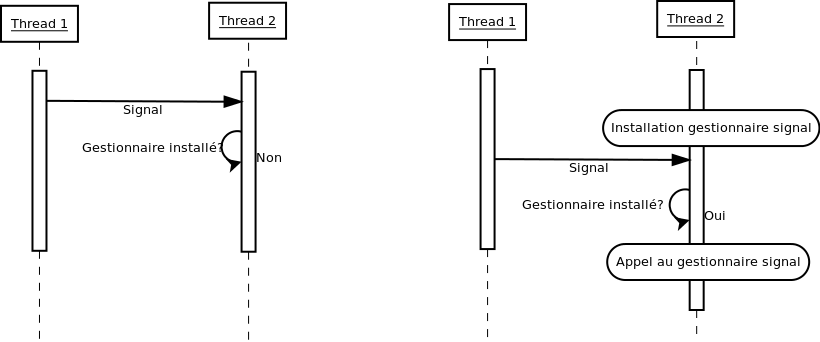
\includegraphics[scale=0.4]{signal.png}
\end{figure}


\subsection{Tests effectués}
Afin de tester cette nouvelle implémentation de signal, le programme \emph{07-signal-test} a été mis en place. 
\paragraph{Avec l'implémentation mise en place}
Le thread \texttt{main} crée tout d'abord un second thread qui va lui envoyer deux signaux successifs. Le gestionnaire n'étant pas installé, les signaux ne sont pas traités quand le thread \texttt{main} reprend la main. Puis, le gestionnaire de ces signaux est installé sur le \texttt{main} et le \texttt{main} créé un troisième thread lui renvoyant les deux signaux. Celui-ci traite le plus prioritaire comme prévu initialement. 

\paragraph{Avec pthread}
En relançant le test avec pthread, nous pouvons obtenir des résultats différents qui dépendent certainement du comportement de la fonction \texttt{signal}. Prenons par exemple, le résultat suivant :\\
> je suis le thread chef :: 0xb75436c0 \\
> je suis le thread 0xb7542358 et je vais envoyer le signal 4 à 0xb75436c0 \\
> je suis le thread 0xb75436c0 et je suis de retour dans le main \\
> je suis le thread 0xb7542358 et je vais envoyer le signal 8 à 0xb75436c0\\
> je suis le thread 0xb6d41358 et je vais envoyer le signal 4 à 0xb75436c0\\
> je suis vraiment le thread 0xb75436c0 et j'ai reçu le signal 8\\
> je suis le thread 0xb6d41358 et je vais envoyer le signal 8 à 0xb75436c0\\
> je suis vraiment le thread 0xb75436c0 et j'ai reçu le signal 8\\
> je suis vraiment le thread 0xb75436c0 et j'ai reçu le signal 4\\
> je suis vraiment le thread 0xb75436c0 et j'ai reçu le signal 4\\

Les signaux 4 et 8 sont traités. En effet, \texttt{pthread} traite tous les signaux reçus dans l'ordre des priorités. De plus, les deux premiers signaux non reçus avec notre implémentation sont également gérés. \\
En effet, les changements de contexte entre les deux threads sont ici plus fréquents. Ainsi, le thread est créé et est désordonnancé avant d'envoyer les signaux, ce qui permet au thread main d'installer le gestionnaire puis de redonner la main au thread qui va lui envoyer les signaux. \\
Le gestionnaire est donc toujours installé avant la réception des messages. Cependant, selon les lancements, la réception des derniers signaux diffère. Ici, le dernier signal 4 ne devrait pas être prise en compte. L'explication pourrait se trouver dans l'implémentation de la fonction \texttt{signal}, qui est dépréciée. 

\paragraph{Conclusion du test}
Ce test a le mérite de montrer que mélanger des signaux et du multithreading requiert une réflexion sur l'influence de l'ordonnancement sur le programme codé. Par ailleurs, il met en évidence les limites de la fonction \texttt{signal} à laquelle il faudrait préférer \texttt{sigaction}.%magnifique !

\subsection{Améliorations possibles}

\paragraph{}
A l'image de \texttt{p\_thread}, l'idée serait de traiter l'ensemble des signaux reçus dans l'ordre des priorités pour éviter une perte de l'information diffusée. Il faudrait donc appeler tous les gestionnaires de signaux reçus, pas seulement le prioritaire. La difficulté reposerait alors sur le comportement du programme si un thread traitant un signal se fait désordonnancer alors que le reste des signaux n'ont pas encore été traités.

\paragraph{}
Par ailleurs, les signaux SIGSTOP et SIGKILL ne doivent normalement pas admettre de gestionnaire. Cette amélioration peut être implémenté en imposant un gestionnaire par défaut à SIGKILL par exemple qui s'occuperait de tuer le thread courant. 

\paragraph{}
Enfin, dans le cas où notre programme aurait plusieurs threads noyaux, il pourrait être imaginé une communication hiérarchique par le biais de signaux uniquement possibles entre les threads noyaux, et d'autres entre les threads noyaux et utilisateur. De plus l'ordonnanceur pourrait alors se permettre lors de la réception d'un signal d'exéctuer le thread destinataire immédiatement.


\section{Préemption}

\paragraph{}
L'utilisateur ne souhaite vraisemblablement pas devoir réfléchir aux endroits où il doit placer des appels à \texttt{thread\_yield()} pour que ses différents threads se partagent équitablement le temps d'exécution.

\paragraph{}
Pour lui éviter d'avoir à s'en soucier (mais aussi éviter qu'un thread partant accidentellement en boucle infinie bloque totalement le programme), un système de préemption est mis en place : les threads sont systématiquement interrompus après un court intervalle de temps s'ils n'ont pas eux-mêmes appelé \texttt{thread\_yield()}.

\subsection{Mise en oeuvre}

\paragraph{}
Le module chargé de la préemption contient cinq fonctions :

\begin{itemize}
\item \texttt{thread\_preemption\_init()}, qu'il faut appeler exactement une fois pour utiliser la preemption. Elle est appelée depuis \texttt{thread\_init()} qui est automatiquement exécutée au démarrage du programme (syntaxe \_\_attribute\_\_((constructor)) de gcc).
Elle alloue et initilalie un timer de la bibliothèque système lequel va nous envoyer périodiquement le signal SIGALARM, et met en place le \textit{signal handler} \texttt{preempt} pour le signal SIGALRM.
\item \texttt{thread\_preemption\_quit()}, symétrique à init, qui désalloue ce que la permière a alloué ; on y fait appel depuis \texttt{thread\_quit()}
\item \texttt{preempt()} est un gestionnaire de signal, qui, sur réception d'un signal d'alarme, appelle \texttt{thread\_yield()} pour donner la main à un autre thread si la préemption est activée.
\item \texttt{thread\_preemption\_enable()} active la préemption (il s'agit simplement de passer à vrai un booléen).
\item \texttt{thread\_preemption\_disable()} la désactive.
\end{itemize}

\paragraph{}
Les deux dernières fonctions permettent d'éviter, typiquement, que l'exécution soit préemptée en plein milieu d'un swapcontext, ou pendant la création d'un thread, ce qui peut avoir des conséquences désastreuses (par exemple essayer de passer la main à un thread dont la pile n'a pas encore été allouée).

\paragraph{}
Pour protéger les appels à \texttt{swapcontext()} tout en s'assurant que la préemption soit toujours activée pendant l'éxécution du code utilisateur, l'invariant suivant est introduit sur les contextes sauvegardés : la prochaine instruction qu'ils éxécutent doit toujours être un appel à \texttt{thread\_preemption\_enable()}.

\paragraph{}
Pour ce faire, les appels à \texttt{swapcontext()} sont immédiatement suivis d'appels à \texttt{thread\_preemption\_enable()} (le contexte qu'on sauvegarde aura donc bien comme prochaine instruction l'activation de la préemption). D'autre part, \texttt{thread\_create()} crée des contextes qui appellent \texttt{thread\_preemption\_enable()} avant d'exécuter la fonction de démarrage du thread.

\subsection{Test}

\paragraph{}
Le test est le suivant : le thread principal crée un thread chargé d'exécuter une boucle infinie sans appel à \texttt{thread\_yield} et lui donne la main. Si la préemption fonctionne, la boucle infinie est préemptée et le thread principal récupère la main. On réitère dix fois pour être bien sûrs du résultat. Le test ne passe effectivement pas sans préemption (il reste coincé dans la boucle infinie). Ce test ne serait plus tout à fait sûr si notre fonction \texttt{thread\_yield()} ne garantissait pas de donner la main à un autre thread que soi-même, s'il en existe un.

\subsubsection{Changements préconisés}

\paragraph{}
On peut actuellement reprocher deux choses à notre implémentation.
Pendant que la préemption est désactivée, le handler continue d'être exécuté pour ne rien faire, gaspillant ainsi une part infime du temps processeur. Il serait peut-être plus efficace d'enlever le \textit{signal handler} pour la désactiver, ou bien (mieux encore) de désactiver le timer, mais nos tentatives en ce sens ont généré des erreurs et nous n'avons pas exploré plus avant ces options.

\paragraph{}
D'autre part, un thread qui ferait de nombreux appels aux fonctions de notre bibliothèque qui désactivent la préemption pendant leur exécution risque de ne jamais être préempté si à chaque SIGALRM reçu l'exécution est au milieu d'une de ces fonctions.
On peut facilement pallier ce problème en ajoutant un appel à \texttt{thread\_yield} dans les fonctions en question.

\paragraph{}
Dernier détail, la préemption reste active lorsqu'il n'y a qu'un seul thread, et fait des appels inutiles à \texttt{thread\_yield}.




\section{Annulation d'un thread}

\paragraph{}
L'objectif de cette fonctionnalité est de reproduire une fonction analogue à \texttt{pthread\_cancel}, c'est-à-dire de pouvoir stopper l'exécution d'un autre thread.

\subsection{Mise en oeuvre}

\paragraph{}
Cette fonctionnalité est séparée en deux fonctions:
\begin{itemize}
\item \texttt{thread\_setcancelstate()}, permet d'activer ou de désactiver la possibilité d'annuler un thread, pour éviter divers problèmes d'exécution. Cette fonction manipule un champ de la structure thread : \texttt{is\_cancelable}. Notons qu'une correspondance est faite avec la fonction de \texttt{p\_thread} : mêmes arguments (ancien état et nouveau), et ne peuvent valoir que les deux macros que cette bibliothèque définit.
\item \texttt{thread\_cancel()}, permet d'annuler un thread, elle change simplement le champ \texttt{to\_cancel} du thread à 1. Par la suite, lors d'un yield, on vérifie les champs \texttt{to\_cancel} et \texttt{is\_cancelable}, et s'ils sont valides, le thread est effetivement annulé. Il en est de même dans \texttt{thread\_join}.
\end{itemize}

\paragraph{}
Il convient de préciser dans le fonctionnement de l'annulation, que si un thread a été annulé alors qu'il n'autorisait pas l'annulation, cette demande est gardée en mémoire jusqu'à ce qu'il autorise l'annulation. Par ailleurs la valeur de retour du thread est alors la macro \verb!PTHREAD_CANCELED!, définie par la bibliothèque \texttt{p\_thread}.

\subsection{Tests}

\paragraph{}
Un seul test est destiné à vérifier le bon comportement de la bibliothèque du projet. Il s'agit de \texttt{17-thread-cancel}. Son fonctionnement est assez simple : il consiste à créer un nouveau thread (qui d'abord interdit son annulation puis l'autorise), puis lui envoyer une demande d'annulation. Pour s'assurer du bon fonctionnement, il faut donc que la demande d'annulation soit envoyée pendant que le thread est encore dans l'état où il interdit son annulation.

\paragraph{}
Afin que l'annulation soit requise au bon moment, le principe de base est de faire un \texttt{sleep} afin de laisser un certain laps de temps entre le moment où l'annulation est interdite puis autorisée. Seulement cette technique n'est pas compatible avec la bibliothèque du projet qui ne se base que sur un seul thread utilisateur, et quelques \texttt{thread\_yield()} ont donc été rajoutés. 

\subsection{Ordonancement}

Afin de mieux gérer l'utilisation des threads, une option a été rajoutée afin de prendre en compte la volonté de l'utilisateur de rajouter son thread en tête ou en fin de liste lors d'un yield. Cela consiste donc formellement à considérer la \emph{ready\_list} comme une FIFO ou une LIFO.

\subsection{Fonctionnement}

\paragraph{}
Le fonctionnement de cet avancement est très simple : lors de la création d'un thread par la nouvelle fonction \texttt{thread\_create\_a(..., int a)} qui prend en argument supplémentaire un entier désignant la politique d'ordonnancement voulue (0 pour FIFO, 1 pour LIFO), un champ particulier de la structure du thread est initialisé avec cet entier. Lors de tout ajout à la \emph{ready\_list}, cet entier servira à déterminer s'il faut le mettre en début (LIFO) ou en fin (FIFO) de liste.

\paragraph{}
Afin d'assurer la cohérence avec la fonction originale de création de thread, l'ancienne fonction de création se contente d'appeler la nouvelle avec comme politique FIFO. Le fait qu'il n'y ait pas d'attente infinie est assurée à la fois par la préemption, et à la fois par le fonctionnement de \texttt{thread\_yield()} qui retire sélectionne le premier élément de la liste avant d'ajouter celui qui vient d'être préempté.

\paragraph{}
Notons que cette nouvelle fonction est remplacée par un appel standard de création de thread (sans attribut particulier) dans la bibliothèque \texttt{p\_thread}.

\subsection{Tests}

\paragraph{}
Le principal test effectué est la modification de \texttt{51-fibonacci} qui utilise maintenant une politique LIFO. Le résultat est non seulement une légère amélioration du temps d'exécution, mais aussi et surtout le fait qu'il est alors possible de calculer fibonacci sur n'importe quel entier : il n'y a plus de swap dû au trop grand nombre de threads créés. Maintenant chaque thread créé s'exécute tout de suite et les seuls threads pouvant s'exécuter à sa place sont ceux qu'il vient lui-même de créer, jusqu'à ce que ceux-ci terminent.

\subsection{Améliorations}

\paragraph{}
La principale amélioration consisterait à implémenter des notions de priorités entre les threads, cela nécessiterait plusieurs listes de threads prêts différentes, ainsi qu'une fonction de tri de ces listes. La complexité générale de l'exécution risquerait toutefois d'être trop grande et de la ralentir. 


\section{Validation des résultats}

La validation des résultats consiste principalement en une comparaison entre le comportement de le bibliothèque implémentée lors du projet et celui de \texttt{p\_thread}. Il convient à la fois de vérifier la correspondance des résultats, mais aussi d'expliquer les différences de temps de calcul entre les deux bibliothèques pour des tests choisis. 

\subsection{Scripts de tests}

\paragraph{}
Trois scripts permettent de tester les tests fournis, ainsi que ceux implémentés dans le cadre du projet. 

\paragraph{\texttt{run\_tests.sh}}
Ce script lance tous les tests et effectue un \texttt{diff} entre les sorties des binaires utilisant \texttt{p\_thread} et celles des binaires utilisant la bibliothèque du projet. Les \texttt{diff} ne devraient rien afficher en dehors des différences dues au temps d'exécution ou aux adresses.

\paragraph{\texttt{valgrind\_tests.sh}}
Le principe est identique au script précédent, il ds'agit cette fois de comparer les sorties de valgrind.

\paragraph{\texttt{bench/create\_graph.sh}}
Les tests fournissant leur temps d'exécution en sortie sont ici exécutés afin de comparer les performances des deux bibliothèques. Cinq graphiques sont automatiquement générés, en faisant une moyenne sur dix lancements. Cela permet de s'assurer de la pertinence des performances sur des plateformes différentes.

\subsection{Passage des tests}

\paragraph{Tests fournis}
Tous les tests fournis par M. Goglin fonctionnent avec la bibliothèque implémentée \texttt{thread.so}. Aucune erreur mémoire ne se présente pour ces tests (aucune fuite mémoire, aucune erreur de lecture). \textsf{Valgrind} détecte cependant un changement de pile (et émet un avertissement). Mais cette manipulation est maîtrisée : elle permet en effet de désallouer correctement la pile dans le test \texttt{12-join-main}.

\paragraph{Tests implémentés/modifiés}
La logique des tests implémentés dans le cadre du projet était de vérifier l'exécution des nouvelles fonctionnalités. Ceux-ci ont déjà été présentés dans les sections de ces nouvelles fonctionnalités, notons simplement que leur exécution ne provoque pas non plus d'erreur ni de fuite mémoire.

\paragraph{Rapidité de la bibliothèque du projet}
Les graphiques générés automatiquement par le script dans \texttt{bench/} permet de s'assurer qu'en toute circonstance, la bibliothèque du projet permet une exécution plus rapide des tests. Cela est toutefois a relativiser avec le fait que les tests ne sont pas prévus pour effectuer des opérations parallèles, où seuls une implémentation de threads noyaux aurait pu permettre à la bibliothèque d'être peut-être aussi performante.


\section*{Conclusion}
\paragraph{}
Ce projet a permis à l'ensemble de l'équipe de consolider des bases au niveau de la compréhension du fonctionnement des threads et de leurs interactions. Le fait d'implémenter leur structure depuis l'origine est sans aucun doute la meilleure façon de comprendre le système. Enfin, la comparaison entre pthread et notre bibliothèque a apporté une vision critique au projet en soulevant les avantages des deux entités et en assimilant leurs limites.  
\paragraph{}
Nous regrettons toutefois de ne pas être parvenus à la gestion de plusieurs threads noyaux, qui bien qu'étant une partie très compliquée, soulève des problèmes au moins aussi intéressants que ceux que nous avons abordés.

\end{document}
